\documentclass[12pt]{scrartcl}
\usepackage[sexy]{evan}
\usepackage[noend]{algpseudocode}
\usepackage{answers}
\usepackage{tikz}
\usepackage{tkz-euclide}
\usepackage{listings}
\usepackage{color}
\usepackage{caption}
\usepackage{setspace}
\usepackage{float}
\usepackage{braket}
\usepackage[noend]{algpseudocode}
\usepackage{sansmath}   
\usepackage{pgfplots}
\usepackage{longtable}
\usepackage[top=3cm,left=3cm,right=3cm,bottom=3cm]{geometry}


\newcommand{\U}{\mathcal{U}}
\newcommand{\E}{\mathbb{E}}
\newcommand{\F}{\mathcal{F}}
\newcommand{\R}{\mathbb{R}}
\newcommand{\ra}{\rightarrow}
\newcommand{\eqdef}{=\vcentcolon}
\renewcommand{\O}{\mathcal{O}}
\renewcommand{\solutionextension}{out}

\usetikzlibrary{arrows}
\usetikzlibrary{automata}
\usetikzlibrary{positioning}  %                 ...positioning nodes
\usetikzlibrary{arrows}       %                 ...customizing arrows
\setlength\parindent{0pt}
\newcounter{casenum}
\newenvironment{caseof}{\setcounter{casenum}{1}}{\vskip.5\baselineskip}

\begin{document}
\doublespacing

\title{Vehicle Routing Problem with a Helper}
\author{Ekesh Kumar \\ Bruce L. Golden}
\date{\today}

\maketitle
\tableofcontents
\newpage

\section{Introduction}
\subsection{Preliminaries}
National postal services seek to minimize the makespan of their deliveries by designing optimal routes for their vehicles. The \textit{vehicle routing problem} (VRP) is an optimization problem in operations research in which one seeks to find an optimal set of routes for a fleet of vehicles. Vehicles spend time traveling to predefined service stops and spend a predefined amount of time at each service stop to satisfy a customer's demands. Variants of the vehicle routing problem seek to minimize differing objective functions such as the sum of the route lengths or the makespan of the routes. \\

In this paper, we explore a variant of the vehicle routing problem --- the \textit{vehicle routing problem with a helper} (VRPWH). Instead of having a fleet of vehicles, this problem studies the case in which a single truck driver and a helping agent (a human or robot) work together to provide service at a set of service stops. More precisely, the VRPWH problem has a single \textit{truck driver} who drives a \textit{delivery truck}. The truck driver works with a \textit{helping agent} that can either ride in the delivery truck with the truck driver or travel by foot by themselves. The driver of the delivery truck and the helping agent seek to visit and service a set of predefined service stops $S$ along a long path. We impose the additional constraint that the helping agent walks at a constant factor $\alpha$ slower than the delivery truck. That is, if the delivery truck travels at a speed of $v$, then the helping agent walks at a speed of $\frac{v}{\alpha}$. Furthermore, we impose the additional constraint that the helping agent is only permitted to service a fixed subset $S' \subseteq S$ of service stops that is known ahead of time. \\ % reword

We explore a few well-performing heuristics and metaheuristics for the problem at hand. Although this paper focuses on the case in which there is exactly one helping agent, the heuristics discussed in this report can easily be generalized to two or more helping agents.

\subsection{Past Work}
In $2008$, [1] Rhodes et al. proposed an idea about having a helper dispatch tool for UPS's delivery system. The authors delineate how the decision tool could have a direct impact on savings while also providing a more efficient delivery solution. However, the authors do not mention any routing decisions that can be applied in practice.  \\

In $2017$, [2] Lu introduced the dependent driver helper dispatching problem (DHDP), a related problem that ``had never been studied before." The DHDP problem is similar to the vehicle routing problem problem: It seeks to minimize the cost required to service a set of customers with the assistance of a helper. The driver and helper can share the delivery workload. Furthermore, the DHDP problem is similar to the VRPWH problem as both problems impose the constraint that the helping agent cannot move on its own. However, the DHDP problem differs from the VRPWH problem in that the helping agent is less efficient at providing service to service stops than the truck driver. This is not the case in the VRPWH problem in which the truck driver and the helping agent require the same amount of time to provide service at a fixed service stop. The DHDP problem also differs in that the demands at a service stop can be split among both the primary driver and the helper. This is not permitted in the VRPWH problem --- the truck driver or the helping agent must spend an uninterrupted amount of time to finish providing service at a service stop. Finally, Lu [2] only presents a single heuristic for the DHDP problem in the general case. In our paper, we provide several heuristics specialized for the case in which the underlying tour resembles a circle.


\section{Problem Definition}
\subsection{Assumptions and Constraints}
Consider a mail route with a vehicle that makes numerous stops along a path. At each stop, the mail carrier exits the vehicle and delivers mail to a set of customers clustered along a closed walk on foot. After delivering the mail, the mail carrier returns to his vehicle and continues along the path. Once the truck driver and the helping agent have finished servicing all of the customers, they must return to their initial starting point. \\ % Reword.

In this problem, we seek to find the minimum time required to satisfy customers demands and return to the starting point with the assistance of a helping agent. \\

\noindent We can model the problem by representing the $n$ service stops as points $p_1, p_2, \ldots, p_n$ on a circular path in the real plane. With this circular representation, an instance of the VRPWH problem is fully defined by the following parameters:

\begin{enumerate}
    \item An radius parameter $r$, which is used to describe the circumference of the underlying circle.
    \item A set of service stops $S = \{p_1, \ldots, p_n\}$, where $p_i$ denotes the location of the $i^{\text{th}}$ service stop.
    \item A time function $t : S \mapsto \mathbb{R}$, which maps each service stop to the number of time units required to service the customer at that stop.
    \item A parameter $\alpha$ used to describe the factor by which the helping agent's walking speed is slower than the truck driver's driving speed. In other words, if the truck drives at a speed $v$, then the helping agent's walking speed is $v/\alpha$.
    \item A subset $S' \subseteq S$ of service stops describing where the helping agent can be utilized. If $S' = \emptyset$, then the helping agent cannot be used at all. Conversely, if $S' = S$, we can employ the helping agent at any service stop. 
\end{enumerate}


We impose the following additional constraints: 

\begin{enumerate}
    \item The locations of the service stops are known ahead of time. 
    \item The time required to service each customer is known ahead of time.
    \item The truck in which the truck driver and the helping agent begin in starts at the point $p_0 = (-r, 0)$. 
    % \item The helping agent can walk to different service stops on its own. That is, it is not necessary for the helping agent to travel in the vehicle with the truck driver. However, walking is slower than driving by a factor of $\alpha$. In other words, if the truck drives at a speed $v$, then the helping agent's walking speed is $v/\alpha$.  
    % \item The helping agent might not be able to service a particular customer. For a fixed instance of the VRPWH problem, there is a fixed subset $S' \subseteq S$ of the service stops at which the helping agent can be utilized for service. This means that the truck driver must service the customers at every service stop in $S \setminus S'$. 
    \item The process of serving a customer cannot be split. At every service stop $u \in S$, either the truck driver or the helping agent must spend exactly $t(u)$ uninterrupted time units servicing the customer to completion. 
    \item The truck that the truck driver drives can only move in one of two directions (clockwise or counterclockwise) but not both. We assume a one-way street. On the other hand, the helping agent is able to walk in either direction.  
\end{enumerate}

An example of an instance of the VRPWH problem with parameter $r = 1$ is depicted in Figure 1: 

% Figure
\begin{figure}[H]
\centering
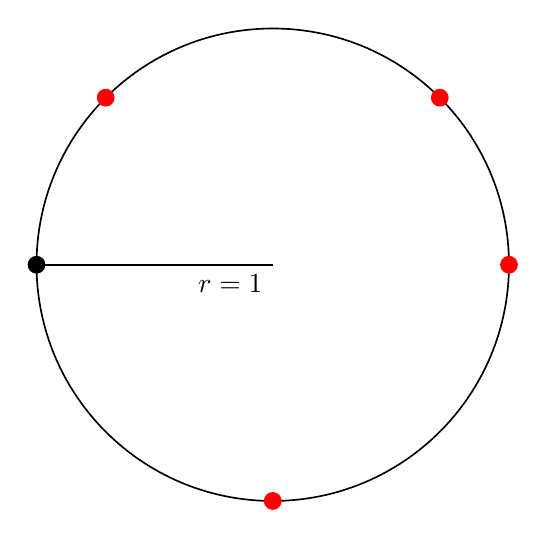
\begin{tikzpicture}[scale=3]
  \draw[semithick] (0,0) circle (1);
  \draw[thick] (-1, 0) -- (0, 0) node[below left] {$r = 1$};
  \draw[black,fill=black] (-1, 0) circle[radius=1pt];
 
  % Service stations
  \draw[red,fill=red] ({sqrt(2)/2}, {sqrt(2)/2}) circle[radius=1pt];
  \draw[red,fill=red] ({-sqrt(2)/2}, {sqrt(2)/2}) circle[radius=1pt];
  \draw[red,fill=red] (1, 0) circle[radius=1pt];
  \draw[red,fill=red] (0, -1) circle[radius=1pt];
\end{tikzpicture}
\caption{VRPWH Problem Instance}
\end{figure}

\noindent In this figure, the starting location of the truck is marked by a solid black dot. There are four service stops whose locations are marked with solid red dots.\\


For notational convenience, we define the following functions:

\begin{enumerate}
    \item $CW : S \mapsto S$ maps a service stop to the next service stop in the clockwise direction. 
    \item $CCW : S \mapsto S$ maps a service stop to the next service stop in the counterclockwise direction.
\end{enumerate}


\iffalse
Another interesting situation is when the vehicle's route is a line. We can model this situation by having the vehicle start at a single point on the real number line. Service stops are scattered along the number line. The vehicle travels towards the end of the number line while servicing some subset of the customers. Afterwards, it travels back to where it started on the number line, possibly servicing a different subset of customers on its way back. \\

The last two cases that are interesting to consider are when the underlying graph that the vehicle traverses is a tree, and the general case in which there is no pre-defined structure for the distribution of the service stops. In either of these cases, we can represent the vehicle's starting point and the service stops it must visit as vertices in a graph. The distances between any two vertices is represented by the weight between the two edges. \\
\fi

\subsection{Hardness}
We now present a proof demonstrating that the VRPWH problem is at least NP-Hard:

\begin{proposition}
The VRPWH Problem is at least NP-hard. 
\end{proposition}
\begin{proof}
Consider an instance of the $\mathsf{PARTITION}$ problem in which we are given a multiset of positive integers $S = \{a_1, \ldots, a_n\}$, and we are tasked with deciding whether or not $S$ can be partitioned into two subsets $S_1$ and $S_2$ such that the sum of the numbers in $S_1$ equals that of $S_2$. It is well-known that $\mathsf{PARTITION}$ is an NP-Hard problem. \\ 

We will demonstrate that the VRPWH on a Circle is also NP-hard by reducing an arbitrary instance of $\mathsf{PARTITION}$ to an instance of the VRPWH on a Circle. \\

Consider an instance of $\mathsf{PARTITION}$ in which we are provided with a multiset of positive integers $S = \{a_1, \ldots, a_n\}$. We wish to determine whether $S$ can be decomposed into the disjoint union of two multisubsets $S_1$ and $S_2$ such that $\sum_{a_i \in S_1} a_i = \sum_{a_j \in S_2} a_j$. We construct an instance of the VRPWH on a Circle whose optimal solution will yield such a partitioning. \\

Construct an instance of the VRPWH on a Circle in which the underlying circle has radius $r$, and we have $n$ service stops with service times $a_1, \ldots, a_n$. In the limit as $r \to 0$, the time required to go around the circle approaches zero. Furthermore, as $\alpha \to 1$, the helping agent's walking speed approaches that of the truck driver's driving speed. In other words, there is no advantage in having the helping agent dropped off at the service stops it visits over having the helping agent walking to that service stop on its own. \\

Thus, an optimal solution to such an instance of the VRPWH on a Circle becomes one in which the customers' demands are divided evenly. In other words, if $T_1$ denotes the time that the truck driver spends servicing customers and $T_2$ denotes the time that the helping agent spends servicing customers, then an optimal solution to the VRPWH on a Circle instance minimizes the quantity $|T_1 - T_2|$. By definition, the two multisubsets of $S$ that attain the sums $T_1$ and $T_2$ form an optimal solution to the corresponding $\mathsf{PARTITION}$ instance. 
\end{proof}

\section{Properties of Efficient Solutions}
When designing efficient heuristics for the VRPWH on a Circle, we take several observations into account. First, we present a few loose upper bounds for the problem at hand. Next, we introduce several strategies that are weakly dominated (i.e., there is always another course of action that is at least as good as that strategy). \\

By taking these bounds and dominated strategies into consideration, we can significantly reduce the search space for an efficient solution. 

\subsection{Bounds}

\begin{proposition}
Consider an instance of the VRPWH on a circle in which the underlying circle has radius $r$. Let the $n$ service stops be $a_1, \ldots, a_n$ with respective service times $t(a_1), t(a_2), \ldots, t(a_n)$. No solution to the VRPWH will take less than $2\pi r + \frac{1}{2}\sum_{i} t(a_i)$ time.
\end{proposition}
\begin{proof}
If the truck driver were to service every customer by himself, he would spend a total of $\sum_{i} t(a_i)$ time. However, if this process were fully parallelized with the helping agent (i.e., for every time unit spent by the truck driver servicing a customer, the helping agent also spends a time unit servicing a customer), they would spend a total of $\frac{1}{2} \sum_{i} t(a_i)$ elapsed time units. This does not include any travel costs, which can only make this number increase. In particular, one can note that the travel costs will always be \textit{at least} $2\pi r$ as the truck driver can only move in one direction meaning that it must go around the circle at least once. Thus, we conclude that no solution to an instance of the VRPWH on a circle will ever take less than $2\pi r + \frac{1}{2}\sum_{i} t(a_i)$ time. 
\end{proof}

With this result in mind, we seek to find efficient heuristics and results that will allow us to approximate an optimal solution in a computationally feasible manner.


\subsection{Dominated Strategies}

\begin{proposition}
[Dominated Strategies: Helping Agent Idleness]
It is never advantageous for the helping agent to remain idle. For each solution in which the helping agent remains idle, there is a corresponding solution that can possibly upon the initial solution in which the helping agent always spends his time moving (possibly in the truck) or servicing a customer.
\end{proposition}
\begin{proof}
Consider an instance of the VRPWH on a Circle. Let $\mathsf{IDLE}$ denote a feasible solution in which the helping agent remains idle for a non-zero period of time. We will construct a new solution $\mathsf{SOL}$ that performs at least as well as $\mathsf{IDLE}$ in which the helping agent remains idle for exactly zero time units. \\

Consider an arbitrary point in time in $\mathsf{IDLE}$ in which the helping agent remains idle. Let $p_k$ be the next point (either a service stop or the starting point) that the helping agent will visit. We consider two collectively exhaustive cases (the location of the truck driver does not matter):

\begin{enumerate}
    \item The helping agent will walk to $p_k$ on his own. In this case, it is clearly disadvantageous to remain idle. By assumption, the helping agent is not already servicing a customer. Moreover, $p_k$ is the next service stop (or initial point) that the helping agent will visit. By removing the idle time and instead starting to walk to $p_k$ immediately, we obtain $\mathsf{SOL}$, which improves upon $\mathsf{IDLE}$ by exactly the time that the helping agent remained idle before starting to walk to $p_k.$  
		\item The helping agent will be dropped off at $p_k$ by the truck. In this case, we can construct $\mathsf{SOL}$ by removing the idle time of the helping agent and instead have the helping agent walk towards the truck. This is always possible because the helping agent is permitted to walk in both the clockwise and counterclockwise direction. Furthermore, this solution can only improve upon $\mathsf{IDLE}$ since the helping agent cannot walk faster than the truck (i.e., $\alpha \geq 1$).  
\end{enumerate}

\noindent There is one last special case that needs to be considered. Consider the case in which there is no ``next point" $p_k$ that the helping agent needs to visit. This can happen when the helping agent has finished servicing the subset of customers that it was assigned by a feasible solution, and it has returned to the initial starting point on its own. In this case, we can still construct $\mathsf{SOL}$ by having the helping agent walk in the direction that is opposite of the direction that the truck is moving in. Since the truck cannot move in both directions, we are guaranteed that the helping agent will encounter the truck. Once the helping agent encounters the truck, it should ride in the truck with the truck driver for the remainder of the solution. \\

This course of action cannot make the preceding feasible solution any worse since the makespan of the solution is already being limited by the time that the truck driver requires to return back to the starting point. 
\end{proof}

\iffalse
\begin{proposition}
It is never advantageous for the helping agent to walk in the direction opposite to that which that the truck is moving in. 
\end{proposition}
\begin{proof}
TODO. 
\end{proof}
\fi

The next proposition illustrates that it is only optimal for the helping agent to re-enter the truck at a service stop. 

\begin{proposition}
 Suppose the helping agent is no longer in the truck with the truck driver. There is an optimal solution in which the helping agent only re-enters the truck at a service stop.
\end{proposition}
\begin{proof}
Suppose, for the sake of contradiction, that the proposition is not true. In other words, this means that there exists an instance of the VRPWH problem in which it is strictly advantageous for the helping agent to re-enter the truck driver's truck at a point that is not a service stop. \\

Let $a_1, \ldots, a_n$ denote the $n$ service stops, labeled in a clockwise manner around the circle. Suppose the helping agent re-enters the truck between service stops $a_{i}$ and $a_{i + 1}$, where $a_{i + 1}$ is taken to be the starting point when $i = n$. Since the truck can only move in one direction along the circle (either clockwise or counterclockwise), there are exactly two cases to consider. \\

In the first case, we consider the scenario in which the truck is driving towards the helping agent. This means that the helping agent must have walked ahead and ended up in front of the truck at some previous point in time. An optimal solution would only have a helping agent walk ahead if it the helping agent were to service a service stop beyond the truck's current position. However, by Proposition $3.3$, it is never strictly advantageous for the the helping agent to walk backwards after walking ahead. If the helping agent stays where it is after completing the demands at a service stop, the result follows. On the other hand, consider the case in which the helping agent walks forward after completing the demands at a service stop. This can never improve the final solution if the helping agent is being picked up by the truck because the helping agent will always arrive at its subsequent destination at the same time as the truck. Thus, having the helping agent wait at the last service stop it completes results in a corresponding solution that is at least as good as one in which the helping agent walks forward after servicing its last service stop. \\

Next, we consider the case in which the helping agent walks towards the truck. This can only be the case if the helping agent were left behind at some point. An optimal solution would only leave the helping agent behind if it the helping agent was being used to satisfy the demands at some service stop that the truck driver drove past by. By extension, the truck driver must have gone on to service some other customer. If this were not the case, the truck driver would have just serviced the customer that the helping agent was left behind to service. Consider the last customer that the truck driver services prior to the helping agent catching up to the truck. In an optimal solution, it only makes sense for the truck to wait at that last service stop since moving ahead can only increase the gap between the helping agent and the truck (the helping agent's walking speed is less than or equal to the driving speed of the truck). By assumption, we are considering the last service stop prior to the helping agent catching up, which means that we can only decrease the overall time of our solution by having the truck wait at the last service stop that the truck driver processed.



\end{proof}


\subsection{Undominated Strategies}


\begin{proposition}
 Having the truck driver wait is \textit{not} a dominated strategy (i.e., it may be optimal for the truck driver to remain idle).  
\end{proposition}
\begin{proof}
It suffices to construct an instance of the VRPWH problem in which having the truck driver wait is undominated. Consider the following instance in which $\alpha = 1 - \epsilon$ for some suitable choice of $\epsilon > 0$ (i.e., the walking speed of the helping agent is just under that of the driving speed of the truck):

\begin{figure}[H]
\centering
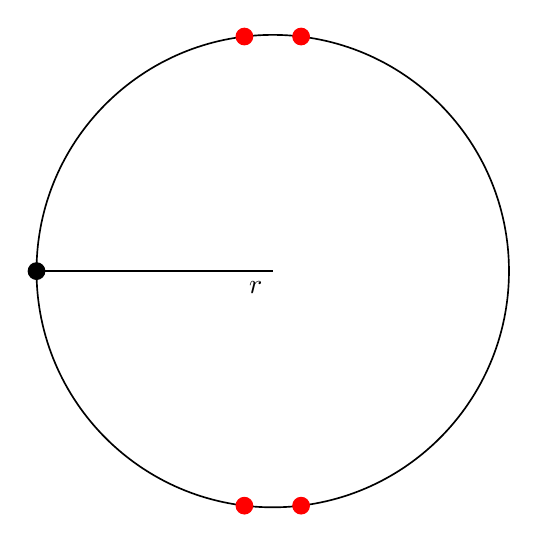
\begin{tikzpicture}[scale=3]
  \draw[semithick] (0,0) circle (1);
  \draw[thick] (-1, 0) -- (0, 0) node[below left] {$r$};
  \draw[black,fill=black] (-1, 0) circle[radius=1pt];
 
  % Service stations
  \draw[red,fill=red] ({-0.12}, {0.993}) circle[radius=1pt];
  \draw[red,fill=red] ({0.12}, {0.993}) circle[radius=1pt];

  \draw[red,fill=red] ({-0.12}, {-0.993}) circle[radius=1pt];
  \draw[red,fill=red] ({0.12}, {-0.993}) circle[radius=1pt];
\end{tikzpicture}
\caption{Primary Deliverer Waiting is Undominated}
\end{figure}
We can label the four service stops in clockwise order as $p_1, p_2, p_3$, and $p_4$. We assume that the helping agent can be utilized at each of the four service stops (that is, $S' = S$). Furthermore, we assume $t(p_i) \ll 2\pi r$, which means that the time required to service the customers is inconsequential when compared to the time required to travel around the circle. \\

With these parameters in mind, consider the following construction of a solution, denoted $\mathsf{IDL}$, in which it makes sense for the truck driver to remain idle:

\begin{itemize}
    \item The truck driver and the helping agent begin at the point $(-1, 0)$, denoted by the solid black circle. They begin to travel in the clockwise direction. 
    \item Upon encountering the first service stop $p_1$, the helping agent is dropped off to service the customers at that station. The truck driver continues along its route in the clockwise direction until it reaches the second service stop, $p_2$. The truck driver services the customer at this second station. 
    \item By construction, we can come up with an instance of the VRPWH problem in which the truck driver and the helping agent finish servicing $p_1$ and $p_2$ at exactly the same time.  
    \item If $r \gg 0$, it would take a notable amount of more time for the helping agent to travel to the next service stop on his own than if it were dropped off by the truck. Furthermore, it would be too costly for the truck driver to make a full lap around the circle to pick up the helping agent. Since the distance between $p_1$ and $p_2$ is relatively small, the merits of having the truck driver wait for the helping agent to arrive at $p_2$ are clear. 
\end{itemize}
\end{proof}



\section{Heuristics}
\subsection{Baseline Heuristic}
To begin our discussion, we introduce a baseline heuristic that does not utilize the helper vehicle at all. The purpose of the baseline heuristic is to simply provide a baseline so that we can easily compare the performance of other heuristics relative to this one. This heuristic is summarized below:

\begin{enumerate}
    \item The truck begins at the point $(-r, 0)$ with the truck driver and the helping agent in the truck. 
    \item While at least one unvisited service stop exists, the truck travels clockwise around the circle to the next unserviced service stop. The truck driver satisfies the demand at the service stop while the helping agent remains idle. 
\end{enumerate}

The baseline heuristic represents the case in which we do not have the option to deploy the helping agent at all. It acts as a ``control" in our subsequent comparisons.  \\

\subsection{Look-ahead Heuristic}
\subsubsection{Heuristic}
The next heuristic we will discuss is called the \vocab{look-ahead} heuristic. The look-ahead heuristic decreases the total time spent by attempting to serve future service stops with the helping agent while the truck driver stays behind to serve a service stop with a large demand. The heuristic is summarized below:

\begin{enumerate}
	\item The truck driver and helping agent both start at the point $(-r, 0)$ on the underlying circle. 
  \item While at least one unvisited service stop exists, the truck travels to the next unserved service stop $a_i$. At $a_i$, we greedily exercise our option to have the truck driver service the customer at $a_i$. Meanwhile, the helping agent ``looks ahead," naively services as many service stops as possible, and returns to $a_i$ in such a way that the truck driver's idle time does not increase at all. 
\end{enumerate}

\subsubsection{Demonstration}
Consider the following instance of the VRPWH on a Circle with $r = 1$ and $\alpha = 1$ in which the locations of the service stops are marked with solid red dots. The starting location of the truck is the solid black dot. For the sake of simplicity, we assume the helping agent can be dispatched at any one of the four service stops. 

\begin{figure}[H]
\centering
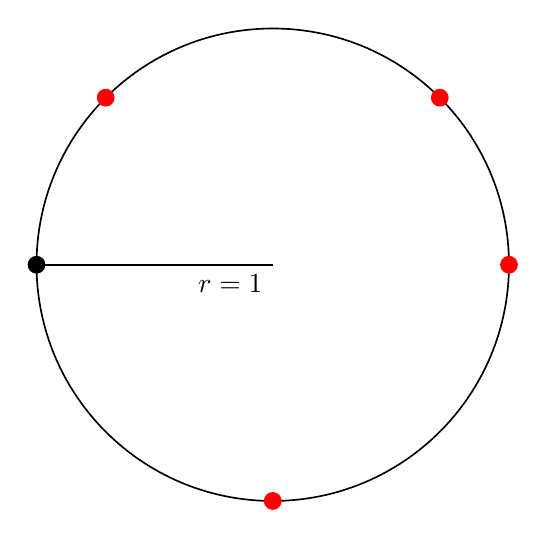
\begin{tikzpicture}[scale=3]
  \draw[semithick] (0,0) circle (1);
  \draw[thick] (-1, 0) -- (0, 0) node[below left] {$r = 1$};
  \draw[black,fill=black] (-1, 0) circle[radius=1pt];
 
  % Service stations
  \draw[red,fill=red] ({sqrt(2)/2}, {sqrt(2)/2}) circle[radius=1pt];
  \draw[red,fill=red] ({-sqrt(2)/2}, {sqrt(2)/2}) circle[radius=1pt];
  \draw[red,fill=red] (1, 0) circle[radius=1pt];
  \draw[red,fill=red] (0, -1) circle[radius=1pt];
\end{tikzpicture}
\caption{Look-ahead Demonstration}
\end{figure}

There are four service stops depicted in the instance above: $a_1 = (-\sqrt{2}/2, \sqrt{2}/2), a_2 = (\sqrt{2}/2, \sqrt{2}/2), a_3 = (1, 0), a_4 = (0, -1)$. Suppose the service times are given by $t(a_1) = 5$, $t(a_2) = 1$,  $t(a_3) = 2$, and $t(a_4) = 20$. Furthermore, suppose that the time required to move a single unit on the Euclidean plane is equal to one time unit. Thus, we spend a total of $2\pi$ time units traveling around the entire circle once. \\

In this instance of the VRPWH on a Circle, the look-ahead heuristic would proceed as follows:

\begin{enumerate}
    \item The truck begins at the point $(-1, 0)$ with both the truck driver and the helping agent. 
    \item The truck travels to the point $a_1$ at a cost of $\pi/4$ time units. We greedily exercise our option to dispatch the truck driver to provide service at this service stop. 
		\item While the truck driver spends $t(a_1) = 5$ uninterrupted time units servicing $a_1$, the helping agent walks $\pi/2$ units to $a_2$, services it in one time unit, travels $\pi/2$ units back to $a_1$, and waits for the helping agent to finish servicing $a_1$. That is, the helping agent ``looks ahead" to see if it can service future service stops while the helping agent stays behind servicing a different service stop. Note that the helping agent cannot service both $a_2$ and $a_3$ without increasing the idle time of the truck driver, so it must return to $a_1$ immediately after servicing $a_2$.  
    \item The truck driver and helping agent travel together to $a_3$ in a total of $5\pi/4$ time units. The truck driver services $a_3$. Since the helping agent cannot service $a_4$ and return to $a_3$ without increasing the idle time of the truck driver, the helping agent remains idle for $t(a_3) = 2$ time units. 
    \item The helping agent and the truck driver travel together in the truck to $a_4$ in a total of $\pi/2$ time units. The truck driver services $a_4$ in $t(a_4) = 20$ time units while the helping agent remains idle. 
    \item Finally, the truck driver and helping agent travel together to their starting point in $\pi/2$ units. All customers' demands have been satisfied, so the heuristic terminates here.
\end{enumerate}

\noindent The total cost of this solution is 
\[
\frac{\pi}{4} + 5 + \frac{3\pi}{4} + 2 + \frac{\pi}{2} + 20 + \frac{\pi}{2} = 27 + 2\pi. 
\]

Despite the straightforward manner of this heuristic, computational results demonstrate that it performs well under certain circumstances. One can note that the total time spent traveling will never exceed $2\pi r$ provided that the time needed to move one unit of distance is equal to one unit of time. \\

The lookahead heuristic improves upon the baseline heuristic by exercising the option to service customers ahead of the one that the helping agent is servicing in such a way that the helping agents' idle time does not increase. Computational results demonstrate that the lookahead heuristic actually manages to exercise this ``lookahead" more than one might expect. For example, the table below demonstrates some of these results for varying radii when the number of service stops is fixed at $100$ and the distribution of demands follows a standard normal distribution. Note, however, that we do not permit negative service times. Thus, if the generated value is below $0$ or above $2\mu$, it is discarded and generated again. This procedure preserves symmetry and ensures demands are non-negative. \\

\noindent The table below depicts the mean number of service stops skipped across $10^{6}$ random instances of the VRPWH on a Circle with a varying radii. In this instance, we assume that the helping agent can service any one service stop with probability $p = 0.50$.


\renewcommand{\figurename}{Table}
\begin{figure}[H]
\centering
\begin{tabular}{ |c|c|c||c| } 
 \hline
 $\#$ of Service Stations & Radius & Mean $\#$ of Skipped Stations \\
 \hline
 $100$ & $1$ & $17.620$ \\ 
 \hline
 $100$ & $2$ & $16.897$ \\ 
 \hline
 $100$ & $5$ & $14.516$ \\
 \hline
 $100$ & $10$ & $11.324$ \\
 \hline
 $100$ & $25$ & $6.508$ \\
 \hline
 $100$ & $50$ & $3.772$ \\
 \hline
\end{tabular}
\caption{Average Number of Skipped Stations in Randomly Generated VRPWH Instances with $p = 0.50$}
\end{figure}
% \renewcommand{\figurename}{Figure}

As demonstrated in the table above, even when the ratio of the number of service stops to the circumference of the circle in the VRPWH instance is small, we can still improve upon the baseline heuristic more than one may expect.

\subsection{Knapsack Look-ahead Heuristic}
\subsubsection{Motivation}
The next heuristic we present is the \vocab{knapsack look-ahead heuristic}, which we motivate through an example. \\ 

Recall that the look-ahead heuristic greedily exercises the option to utilize the truck driver at a service stop whenever possible. The helping agent subsequently serves as many service stops beyond the current one by considering the service stops by considering them in order of their distance to the current service stop. However, this approach may have drawbacks. Consider an instance of the VRPWH on a Circle, and suppose the diagram following represents a small segment of the circle (the curvature of the circle is not depicted here): 

\begin{figure}[H]
  \centering
  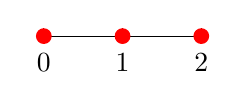
\begin{tikzpicture}
    \draw (0,0) -- (2,0);
    \foreach \i in {0,1,...,2} % numbers on line
      \draw (\i,0.1) -- + (0,-0.2) node[below] {$\i$}; % tick and their labels
    \foreach \i in {0, 1, 2}% points on line
      \fill[red] (\i,0) circle (1 mm);
  \end{tikzpicture}
  \caption{Knapsack Look-ahead Example}
\end{figure}

\noindent For simplicity, assume that the helping agent is allowed to be dispatched at any of the three service stops. Suppose that the time required to satisfy each service stop's demands is given by $t(0) = 10, t(1) = 1,$ and $t(2) = 7$. \\

The look-ahead heuristic would dispatch the truck driver vehicle at $0$. While the truck driver serves this service stop, the helping agent would travel to $1$, service it, and return. The truck driver and helping agent would then travel together to $2$, and the truck driver would service it while the helping agent remains idle. The total cost of the look-ahead heuristic in this instance is $t(0) + 2 + t(2) = 19$ time units. \\

Depending on the value of the parameter $\alpha$, a better solution could be to have the truck driver service the service stop at $0$ while the helping agent travels and services the service stop located at $2$. The helping agent could then return to pick up the truck driver at $0$, they could both travel to $1$, service it, and finally travel to $2$ to finish. The total cost of this solution would be $t(0) + 1 + t(1) + 1 = 13$ time units. \\

In summary, we see that the lookahead heuristic can be improved by not just servicing subsequent service stops in order by their distance to the current service stop but instead servicing subsequent service stops so that the time spent by the primary vehicle is approximately equal to that of the helping agent. Fundamentally, the problem can be reduced to finding a subset of numbers that sum up closest to a target number. 

\subsubsection{Heuristic}
The knapsack look-ahead heuristic operates as follows:

\begin{enumerate}
    \item The truck driver and helping agent begin in the truck located at the point $(-r, 0)$.
    \item The truck driver and helping agent travel together in the clockwise direction. If there is an unserved service stop $a_i$, the truck driver and helping agent travel to it.
		\item We greedily exercise our option to use the truck driver to service the service stop. In the meantime, we ``look ahead" with our primary vehicle, and we service a subset of service stops further in the clockwise direction such that the time spent (round-trip time plus service time) by the helping agent is as close as possible (but not more than) $t(a_i)$. That is, the helping agent's idle time does not increase at all. 
\end{enumerate}

\iffalse
TODO: discuss benefits
\fi


\subsection{Neighbor-Expansion Heuristic}
\subsubsection{Motivation}
The next heuristic we present is the \vocab{neighbor-expansion heuristic}, which is a greedy algorithm that uses some elements from both the look-ahead and knapsack look-ahead heuristics. \\

The preceding two heuristics we discussed both sought to decrease the total time spent by servicing some set of customers by ``looking ahead" with the primary vehicle while the helping agent stayed behind at a particular service stop. \\

Unfortunately, not every optimal solution takes this form. It can be disadvantageous for us to immediately dispatch the truck driver at service stops and only have the helping agent move forward. Consider the following line segment that could be a part of a larger VRPWH on a Circle instance:

\begin{figure}[H]
  \centering
  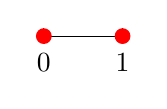
\begin{tikzpicture}
    \draw (0,0) -- (1,0);
    \foreach \i in {0,1} % numbers on line
      \draw (\i,0.1) -- + (0,-0.2) node[below] {$\i$}; % tick and their labels
    \foreach \i in {0, 1}% points on line
      \fill[red] (\i,0) circle (1 mm);
  \end{tikzpicture}
  \caption{Neighborhood-Expansion Example}
\end{figure}

Suppose we have the option to dispatch the helper vehicle at both $0$ and $1$ with $t(0) = 5$ and $t(1) = 15$. Having the truck driver drop the helping agent off at $1$, returning to service stop $0$ and servicing it, and returning to $1$ would produce a solution that takes $16$ time units. On the other hand, both the look-ahead heuristic and the knapsack look-ahead heuristic would take $21$ time units. This demonstrates that it may not always be optimal to ``look ahead" with the primary vehicle while the helper vehicle stays behind. \\

In order to combat the shortcomings of the look-ahead and knapsack heuristics, we propose a new heuristic that considers both ``looking ahead" and ``looking behind" as possible choices. 

\subsubsection{Heuristic}
Before introducing the neighbor-expansion heuristic, we introduce some terminology.

\begin{definition}
For each service stop $a_i \in S$, we define a set of \vocab{neighbors} $N_{a_{i}}$. The set $N_{a_{i}}$ contains the set of service stops for which it is possible for the the helping agent to walk to, service, and return to $a_i$ without exceeding a total time of $t(a_i)$.  
\end{definition}

Essentially, the neighbors of a service stop $a_i \in S'$ represent the set of service stops that the helping agent can potentially service while the truck driver services $a_i$ without increasing the idle time of the truck driver. \\ 

The neighbor-expansion heuristic works as follows:

\begin{enumerate}
    \item We begin with a set $A = \{a_1, a_2, \ldots, a_n\}$ containing every service stop.
    \item While there are service stops in $A$, we perform the following: 
    \begin{enumerate}
        \item For every service stop $a_i \in A$, we compute the set of neighbors $N_{a_{i}}$. 
        \item Next, for each set of neighbors $N_{a_i}$ we compute a subset $N'_{a_i} \subseteq N_{a_i}$ of neighbors such that servicing all of the customers in $N'_{a_i}$ (with travel costs included) is as large as possible but does not exceed $t(a_i)$. This is done in a fashion similar to the knapsack heuristic.
        \item Among all of the computed values, we take the $a_i$ for which the difference between $t(a_i)$ and the time needed to service all of the customers in $N'_{a_i}$ is minimal. Ties are broken arbitrarily. 
				\item We remove both $a_i$ and all of the service stops in $N'_{a_i}$ from $A$, and we repeat this process until $A \cap S' = \emptyset.$ The set $N'_{a_i}$ represents the set of service stops that the helping agent will service while the truck driver services $a_i$. 
    \end{enumerate}
\end{enumerate}

\noindent Upon termination, the set $A$ will be empty. Our solution is constructed as follows:

\begin{enumerate}
	\item The truck driver and helping agent begin at the point $(-r, 0)$ and travel in the clockwise direction.
	\item	When the truck driver and helping agent encounter some service stop $a_i$ that belongs to some $N'_{a_k}$, we should \textit{not} process it immediately. Instead, when we visit $a_k$, the helping agent will be dispatched to service all of the service stops in $N'_{a_k}$. The service stop $a_i$ will be serviced at that point.
	\item When the truck driver and helping agent encounter some service stop $a_i$ that does \textit{not} belong to some $N'_{a_k}$, the service stop $a_i$ should be serviced immediately. 
\end{enumerate}

\subsubsection{Demonstration}
As a brief demonstration, consider an instance of the VRPWH on a Circle with $\alpha = 1$ in which the time required to travel one unit of distance equals one time unit:

\begin{figure}[H]
  \centering
  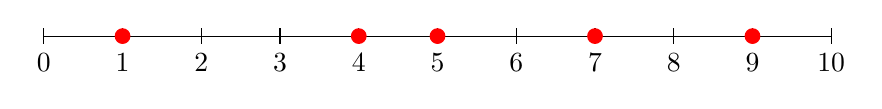
\begin{tikzpicture}
    \draw (0,0) -- (10,0);
    \foreach \i in {0,1,...,10} % numbers on line
      \draw (\i,0.1) -- + (0,-0.2) node[below] {$\i$}; % tick and their labels
    \foreach \i in {1, 4, 5, 9, 7}% points on line
      \fill[red] (\i,0) circle (1 mm);
  \end{tikzpicture}
  \caption{Neighborhood-Expansion Demonstration. Curvature of the circle is not shown.}
\end{figure}

\noindent For simplicity, we assume the helper vehicle can be dispatched at any one of the four service stops. Furthermore, suppose we have $t(1) = 10, t(4) = 7, t(5) = 12, t(7) = 1, t(9) = 1$.  The neighbor-expansion heuristic proceeds as follows:

\begin{enumerate}
    \item First, we initialize $A = \{1, 4, 5, 7, 9\}$ containing the locations of our service stops.
		\item Next, we compute the set of neighbors for each of the four service stops. We have $N_1 = \emptyset$ (the helping agent does not have enough time to travel, service, and return to this service station stop in fewer than $t(1) = 10$ time units), $N_4 = \{7\}, N_5 = \{4, 7, 9\}, N_7 = \emptyset$, and $N_9 = \emptyset$. 
    \item Subsequently, for each $N_{a_i}$, we compute a subset $N'_{a_i}$ of service stops for which the time needed to service all of the customers in $N'_{a_i}$ (with travel costs included) is as large as possible but does not exceed $t(a_i)$. One can find $N'_{1} = \emptyset, N'_{4} = \{7\}, N'_{5} = \{4\}, N_{7} = \emptyset$, and $N_{9} = \emptyset$. Among all of the computed values, we select service stop $4$ since $|t(4) - 3 - t(7) - 3| = 0$. From here, we remove $4$ and $7$ from $A$, and we iterate again. 
    \item In the second iteration, we follow the same procedure, and we end up removing $5$ and $9$ (the other neighbor sets are empty). 
    \item The final solution operates generated by this heuristic operates as follows:
    \begin{enumerate}
        \item The truck driver and helping agent begin at point $0$. 
        \item The truck driver and helping agent move together to $1$ at which the truck driver immediately spends $t(1) = 10$ uninterrupted minutes servicing the customer.
        \item The truck driver and helping agent move together to the service stop at $4$. The truck driver is dispatched here while the helping agent travels to $7$, services $7$, and returns to $4$.
        \item The truck driver and helper agent move together to the service stop at $5$. The truck driver is dispatched here while the helping agent travels to $9$, services $9$, and returns to $5$.
        \item The truck driver and helping agent navigate to $10$. All of the demands have been satisfied. 
    \end{enumerate}
\end{enumerate}


\subsection{Randomized-Expansion Heuristic}
\subsubsection{Motivation}
The computational results in the subsequent section demonstrate that the proposed heuristics already appear to perform much better than the baseline solution. Notably, the knapsack look-ahead and the neighbor-expansion heuristics appear to perform better than the standard look-ahead heuristic. \\

However, this improvement comes at a price: both the knapsack look-ahead and neighbor-expansion heuristics are more involved, and they perform constant-time operations on the same service stop several times. Although the two heuristics appear to perform very quickly when the service stops and service times are generated according to naturally arising probability distributions, step $2$ of either algorithm runs in worst-case exponential time. When working with several service stops, these approaches may be computationally infeasible. \\

This motivates us to seek different approaches. In this section, we present a randomized metaheuristic that is structurally similar to the neighbor-expansion heuristic. However, it speeds up and potentially improves upon the neighbor-expansion heuristic by utilizing stochastic decision making. We refer to this approximation as the \vocab{randomized-expansion heuristic}. 


\subsubsection{Heuristic}

In the knapsack look-ahead and neighbor-expansion heuristics, the process of finding the neighbors of some service stop $a_i \in S'$ is fast (i.e., they can be computed in polynomial time), but computing the desired optimal subset of $S'$. The randomized-expansion heuristic improves upon the latter step by making randomized decisions. \\

The randomized-expansion heuristic works as follows:

\begin{enumerate}
    \item We begin with a set $A = \{a_1, a_2, \ldots, a_n\}$ containing every service stop.
		\item While $A$ is nonempty (i.e., while there are service stops that need to be serviced), we perform the following:
    \begin{enumerate}
        \item For each service stop $a_i \in A \cap S'$, we compute the set of neighbors $N_{a_i}$.
        \item Next, for each set of neighbors $N_{a_i}$, we generate a random subset $N'_{a_i}$ of $N_{a_i}$. If the time required to service all of the service stops (with travel costs included) exceeds $t(a_i)$, we discard the generated subset. This step is guaranteed to terminate because any singleton would satisfy the desired properties.\footnote{The expected number of steps needed to terminate is polynomial in $n$.}. 
        \item For each random subset $N'_{a_i}$, we compute the absolute difference between $t(a_i)$ and the time required to service (with travel costs) each of the service stops in $N'_{a_i}$ and return to $a_i$.
        \item Steps $a, b, c$ are repeated a fixed number of times. Among all of the computed absolute differences, we take the $a_i$ and $N'_{a_i}$ for which the absolute difference was minimal. 
        \item We remove both $a_i$ and all of the service stops in $N'_{a_i}$, and we repeat Step $2$ until $A \cap S' = \emptyset$.
    \end{enumerate}
    \item At this point, we construct a solution as we would in the neighbor-expansion heuristic. 
    \item We can repeat this entire algorithm several times, and we can take the best objective value found from all repetitions. 
\end{enumerate}

Introducing randomness into the expansion heuristic serves two purposes:

\begin{enumerate}
    \item First, we are able to significantly improve the running time of the previous algorithms that we proposed.
    \item Next, there is a high chance that some of the found solutions will differ from what the other proposed algorithms found. These differences are analogous to the concept of mutations in genetic algorithms. 
\end{enumerate}




\iffalse
\subsubsection{Analytical Results}

We will now provide some analytical results on the performance of the look-ahead heuristic when the locations of the service stops and the time required to serve each customer follow fixed probability distributions. \\

Consider an instance of the VRPWH problem with $n$ service stops. Suppose the locations of the service stops $a_1, a_2, \ldots a_n$ are i.i.d. random variables with a $\mathcal{U}(0, L)$ distribution for some fixed constant $L$. Furthermore, suppose that the times required to service each stop $t(a_1), t(a_2), \ldots, t(a_n)$ follow a $\mathcal{N}(\mu, \sigma^2)$ distribution for fixed positive constants $\mu$ and $\sigma$. Furthermore, suppose that each $a_i$ belongs to $S'$, the set of service stops that the helper vehicle can be dispatched at, with probability $p$.  


\begin{lemma}
improves upon the with probability 
\end{lemma}
\begin{proof}
Let $\pi$ be the unique permutation of $\{1, 2, \ldots, n\}$ for which $a_{\pi(1)} < a_{\pi(2)} < \cdots < a_{\pi(n)}$. The look-ahead heuristic does \textit{not} improve upon the baseline heuristic if and only if we never have the opportunity to exercise the option to ``look-ahead" with the primary vehicle. \\

Suppose $|S'| = k$ (i.e., there are exactly $k$ service stops at which we may exercise the option to dispatch the helper vehicle). The probability that we cannot ``look ahead" at some service stop $a_{\pi(i)} \in S'$ is exactly the probability that the event $\{i = n \vee t(a_{\pi(i)}) > 2 \cdot (a_{\pi(i + 1)} - a_{\pi(i)}) + t(a_{\pi(i + 1)})\}$ occurs. This is true because we can never ``look ahead" at $i = n$, and we also cannot look ahead when the time required to service the station at $a_{\pi(i)}$ is longer than the time required to travel to $a_{\pi(i + 1)}$, service it, and return. We can
\[
P(t(a_i) > 2(a_{i + 1} - a_{i}) + t(a_{i + 1})) = P(t(a_i) 
\]
\end{proof}
\fi

\iffalse
\section{Shortest-Path Heuristic}
\subsection{Introduction}
The heuristic we propose involves using the \vocab{depth-first search spanning tree} of the underlying graph that models the problem. \\% 

Consider an undirected graph. The depth-first search traversal of the graph can be implemented by a recursive function that starts at a root node and explores as far as possible along each branch before backtracking. \\ % 

Consider all of the edges that were traversed during the depth-first search traversal of the graph. They form a spanning tree of the graph, rooted at the source node. We call these edges \vocab{span-edges}, and all other edges that were not traversed are called \vocab{back-edges}. The back-edges of the graph all connect a vertex with its descendant in the spanning tree. Note that the term ``tree" in ``depth-first search spanning tree" is slightly misleading as the depth-first search spanning tree can form cycles with its span-edges and back-edges. \\

The depth-first search spanning tree is useful because it significantly simplifies the structure of the underlying graph; we only need to worry about a few ancestor-descendant edges. 
\fi

\iffalse
\section{Dominated Strategies}

\noindent Prior to proposing various heuristics, we note the following observations that must be taken into account when designing our heuristic: 

\begin{quote}
    Suppose we visit a service stop $a_i \in S'$ with the primary and helper vehicles both available. It is never advantageous to service $a_i$ with the primary vehicle since we can instead service $a_i$ with the helper vehicle and possibly satisfy even more demands with the primary vehicle. 
\end{quote}
\fi



\iffalse
\subsection{Analytic Results}

The idle time for the problem cannot be approximated since simply the task of determining whether it is non-zero is strongly NP-hard (reduction to $3$-Partition). However, we claim that the proposed algorithm is an efficient polynomial-time approximation scheme for the makespan of an optimal solution. \\
\fi


\iffalse
\section{Randomized Heuristic}
\subsection{Description}
% \noindent In the previously described deterministic heuristic, we came up with a rule which, upon satisfied, 

\noindent A second heuristic for the VRPWH problem is the following:

\begin{enumerate}
    \item Compute the proportion $p = |V'|/|V|$ of service stops that can be handled by the helper vehicle.
    \item Identify the closest service stop that has not yet been serviced. There are now two cases to consider:
    \begin{enumerate}
        \item If $u\in V'$, then we have the option to handle $u$ with the helper mailman. We generate a $\mathcal{U}(0, 1)$ random variable. If $U \leq p$, then we handle $u$ with the helper vehicle, and we consider the remaining unserviced customers in non-decrasing order by their distance to $u$. We handle as many customers  as possible so that the helper vehicle has zero idle time (i.e., it will never be waiting at $u$ for the primary vehicle to come back).
        \item If $u \not \in V'$, then 
    \end{enumerate}
\end{enumerate}
\fi

\iffalse
\section{Mixed-Integer Program Formulation}
In this section, we present a mixed-integer program (MIP) formulation for the VRPWH problem. This MIP can be used as a first step for developing exact methods to solve the VRPWH problem. Furthermore, it can provide a better lower bound than naive heuristics. This improved lower bound can be utilized to assess the quality of the solutions generated by the proposed heuristics.  \\


A formulation is provided below:

\begin{equation*}
\begin{array}{ll@{}ll}
\text{minimize}  & ct &\\
\text{subject to}&  j\\ &                                                & x_{j} \in \{0,1\}, &j=1 ,\dots, m
\end{array}
\end{equation*}
\fi


\section{Computational Results}
In order to benchmark the proposed algorithms, we generated random instances of the VRPWH on a Circle. For a fixed radius $r > 0$ and a fixed number of points $N$, the locations of the $N$ service stops were generated randomly on the circle $x^2 + y^2 = r^2$. More precisely, this is done by generating a random angle $\theta$ by sampling a uniform random variable $Z \sim U(0, 1)$ and setting $\theta = 2\pi Z$. From here, we can easily find our random point $(x, y)$ on the circumference of the circle by setting $x = r\cos(\theta)$ and $y = r\sin(\theta)$. \\

On the other hand, the service times of the $N$ service stops were generated according to a ``restricted" $N(\mu, \sigma^2)$ distribution in which service times above $2\mu$ or below $0$ were regenerated in order to preserve symmetry and avoid negative service times. In each instance, a parameter $p$ was also specified, which was used to denote the probability of any one service stop belonging to the subset of service stops that the helper vehicle can be dispatched at. Each computed cost is calculated by averaging over $10^{6}$ simulations each. \\

\begin{figure}[H]
\centering
 \begin{longtable}{|c|c|c|c|c|c|c|c|c|c|c|} 
 \hline
 $N$ & $r$ & $p$ & $\mu$ & $\sigma^2$ & $\alpha$ & Baseline & Lookahead & Knapsack & NE & RE \\
 \hline 
  $10$ & $1$ & $0$ & $1$ & $1$ & $1$ & $2.351$ & $1.641$ & $1.476$ & $1.752$ & $1.380$\\ 
 \hline
 $10$ & $1$ & $0.25$ & $1$ & $1$ & $1$ & $2.359$ & $1.624$ & $1.479$ & $1.877$ & $1.291$ \\
 \hline
 $10$ & $1$ & $0.50$ & $1$ & $1$ & $1$ & $2.416$ & $1.681$ & $1.424$ & $1.829$ & $1.400$ \\
 \hline
 $10$ & $1$ & $0.75$ & $1$ & $1$ & $1$ & $2.473$ & $1.760$ & $1.592$ & $1.843$ & $1.452$ \\
 \hline
 $10$ & $1$ & $1$ & $1$ & $1$ & $1$ & $2.465$ & $1.737$ & $1.539$ & $1.821$ & $1.475$ \\ 
 \hline
 $25$ & $1$ & $0$ & $2$ & $1$ & $4$ & $10.173$ & $7.745$ & $7.126$ & $8.076$ & $5.885$ \\
 \hline
 $25$ & $1$ & $0.25$ & $2$ & $1$ & $4$ & $10.6513$ & $8.271$ & $8.425$ & $8.439$ & $6.146$ \\
 \hline
 $25$ & $1$ & $0.50$ & $2$ & $1$ & $4$ & $10.295$ & $7.881$ & $6.095$ & $7.909$ & $5.896$ \\
 \hline
 $25$ & $1$ & $0.75$ & $2$ & $1$ & $4$ & $10.582$ & $8.191$ & $6.794$ & $8.104$ & $6.054$ \\
 \hline
 $25$ & $1$ & $1$ & $2$  & $1$ & $4$ & $10.298$ & $7.871$ & $8.221$ & $7.812$ & $5.945$ \\
 \hline
 $50$ & $1$ & $0$ & $3$ & $1$ & $2$ & $24.523$ & $17.612$ & $16.783$ & $18.724$ & $14.045$ \\
 \hline
 $50$ & $1$ & $0.25$ & $3$ & $1$ & $2$ & $24.345$ & $17.535$ & $15.504$ & $18.625$ & $13.895$ \\
 \hline
 $50$ & $1$ & $0.50$ & $3$ & $1$ & $2$ & $24.659$ & $17.791$ & $15.071$ & $18.925$ & $14.406$ \\
 \hline
 $50$ & $1$ & $0.75$ & $3$ & $1$ & $2$ & $24.485$ & $17.713$ & $15.022$ & $18.723$ & $13.997$ \\
 \hline
 $50$ & $1$ & $1$ & $3$ & $1$ & $2$ & $24.713$ & $17.822$ & $15.191$ & $18.957$ & $14.081$ \\
 \hline
 $75$ & $1$ & $0$ & $5$ & $1$ & $\frac{4}{3}$ & $43.829$ & $26.052$ & $57.642$ & $33.586$ & $24.999$ \\
 \hline
 $75$ & $1$ & $0.25$ & $5$ & $1$ & $\frac{4}{3}$ & $43.905$ & $26.111$ & $24.342$ & $23.610$ & $21.067$ \\
 \hline
  $75$ & $1$ & $0.50$ & $5$ & $1$ & $\frac{4}{3}$ &  $43.905$ & $26.261$ & $25.342$ & $23.614$ & $21.069$ \\
 \hline
 $75$ & $1$ & $0.75$ & $5$ & $1$ & $\frac{4}{3}$ & $43.904$ & $26.923$ & $25.276$ & $23.567$ & $21.109$ \\
  \hline
 $75$ & $1$ & $1$ & $5$ & $1$ & $\frac{4}{3}$ & $43.855$ & $26.051$ & $24.012$ & $23.535$ & $21.079$ \\
 \hline
 $100$ & $1$ & $0$ & $10$ & $1$ & $\infty$ & $83.617$ & $36.012$ & $34.924$ & $32.691$ & $34.950$ \\
 \hline
 $100$ & $1$ & $0.25$ & $10$ & $1$ & $\infty$ & $83.783$ & $35.241$ & $32.792$ & $34.155$ & $33.826$ \\
 \hline
 $100$ & $1$ & $0.50$ & $10$ & $1$ & $\infty$ & $83.698$ & $35.012$ & $31.461$ & $33.950$ & $32.891$ \\
 \hline
 $100$ & $1$ & $0.75$ & $10$ & $1$ & $\infty$ & $83.698$ & $35.212$ & $31.421$ & $32.945$ & $27.121$ \\
 \hline
 $100$ & $1$ & $1$ & $10$  & $1$ & $\infty$ & $78.746$ & $29.521$ & $28.192$ & $43.421$ & $30.991$ \\
 \hline
 \end{longtable}  
 \caption{Performance of Heuristics on Random Instances of the VRPWH Problem. $N$ denotes the number of service stations; $r$ is the radius of the underlying circle; $p$ denotes the probability of a fixed service stop belonging to the subset of service stops that the helping agent can service; $\mu$ and $\sigma^2$ denote the mean and variance of the underlying normal distribution used to generate the service times of each stop; $\alpha$ denotes the constant factor by which the helping agent walks slower than the truck.}
\end{figure}

From the computational results, it is immediately clear that all of the proposed heuristics outperform the baseline heuristic. This is expected since the baseline heuristic does not utilize the helping agent at all; it simply provides us with an initial value that we can use to compare to the other heuristics.  \\

We see that the simple lookahead heuristic always outperformed the baseline heuristic but it never outperformed any of the other heuristic. Despite its poor performance relative to the other heuristics, the lookahead heuristic is not computationally intensive compared to the other heuristics. On the other hand, the knapsack heuristic typically outperforms the lookahead heuristic but it is extremely computationally intensive. This stems from the fact that the knapsack heuristic is a pseudopolynomial dynamic programming algorithm, and its asymptotic runtime grows according to the sum of the service demands. \\

The neighbor expansion heuristic was also computationally intensive; however, it was not nearly as intensive as the knapsack heuristic. On most instances, it seemed to perform worse than both the lookahead and knapsack heuristics. Finally, the randomized expansion heuristic took a Monte Carlo approach, and it seems to perform the best out of all of the proposed heuristics. The running time of the randomized expansion heuristic typically fell between that of the neighbor expansion heuristic and the knapsack heuristic. 

% \section{Extensions (In progress)}

% \subsection{Related Literature}
% \section{Appendix}
\appendix

\newpage

\section*{References}

\begin{enumerate}
    \item Rhodes, K., Nehring, R., Wilk, B., Patel, N. (2007). UPS Helper Dispatch Analysis. In Systems and Information Engineering Design Symposium, 2007. SIEDS 2007. IEEE. 1-6
    \item Lu, Shih-Hao. "Driver helper dispatching problems: Three essays." Iowa State University (2017).
\end{enumerate}
\end{document}
